\documentclass[12pt]{report}
\usepackage[a4paper]{geometry}
\usepackage[myheadings]{fullpage}
\usepackage{fancyhdr}
\usepackage{lastpage}
\usepackage{graphicx, wrapfig, subcaption, setspace, booktabs}
\usepackage[T1]{fontenc}
\usepackage[font=small, labelfont=bf]{caption}
\usepackage{fourier}
\usepackage[protrusion=true, expansion=true]{microtype}

\usepackage[english]{babel}
\usepackage{sectsty}
\usepackage{url, lipsum}
\usepackage{tgbonum}
\usepackage{hyperref}
\usepackage{xcolor}

\newcommand{\HRule}[1]{\rule{\linewidth}{#1}}
\onehalfspacing
\setcounter{tocdepth}{5}
\setcounter{secnumdepth}{5}

\begin{document}
{\fontfamily{cmr}\selectfont
\title{ \normalsize \textsc{}
		\\ [2.0cm]
		\HRule{0.5pt} \\
		\LARGE \textbf{\uppercase{Natural Language Processing}
		\HRule{2pt} \\ [0.5cm]
		\normalsize \today \vspace*{5\baselineskip}}
		}



\author{
        Nikita Masand\\
        Mentor: Prof Pranav Nerurkar \\
		Veermata Jijabai Technological Institute \\ 
		Matunga, Mumbai \\
		Information Technology\\
		ID: 171081054 \\
		}

\maketitle
\tableofcontents
\listoffigures
\listoftables
\newpage

%-------------------------------------------------------------------------------
% Section title formatting
\sectionfont{\scshape}
%-------------------------------------------------------------------------------

%-------------------------------------------------------------------------------
% BODY
%-------------------------------------------------------------------------------

\chapter{Abstract}
Natural Language  Processing (NLP)  is  a way  of analyzing  texts  by  computerized  means. NLP  involves
gathering of knowledge on  how human  beings understand  and use  language. This is  done  in order  to
develop appropriate tools and techniques which could make computer systems understand and
manipulate natural languages to perform various desired tasks. This paper reviews the literature on NLP.
It also  covers or gives a hint  about the history of  NLP. It is  based on document analysis.  This research
paper could be beneficial to those who wish to study and learn about NLP.
\begin{figure}
    \centering
    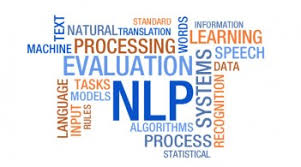
\includegraphics[width=\textwidth]{nlp.jpeg}}
    \caption{NLP}
    \caption*{hackernoon.com}
    \label{nlp1}
\end{figure}
Keywords: NLP, machine translation, machine learning, computational techniques, linguists

\usepackage{graphicx}

\chapter{What is NLP?}
Artificial intelligence (AI) technologies such as machine learning (ML) and deep learning (DL) are dazzling in and of themselves, but believe it or not, leveraged in isolation, they are limited in their potential. These technologies do not interpret data by themselves: they are tied either to deterministic, hard coded software programs created by humans or they are linked to a form of artificial intelligence that can interpret human language into a form ML and DL algorithms can understand. The umbrella term for this gateway AI technology is natural language processing (NLP).\\

Various  researchers  have  explained  Natural  Language Processing  (NLP)  as an  area  of research  and
application that explores how computers can be used to understand and manipulate natural language text
or speech to do useful things
The term NLP is normally
used to describe the function of software or hardware components in a computer system which analyze
or  synthesize  spoken  or  written  language.\\

\section{Understanding Terms in a NLP Project}

The research and development in NLP over the last sixty years as stated by Church and Rau can be
categorized into the following five areas: \\
Natural Language Understanding \\
Natural Language Generation \\
Speech or Voice recognition \\
Machine Translation \\
Spelling Correction and Grammar Checking\\

\begin{figure}
    \centering
    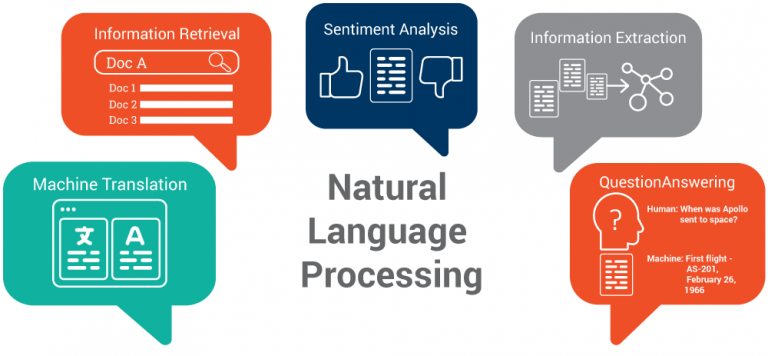
\includegraphics[width=\textwidth]{img.png}
    \caption{Process}
    \caption*{https://miro.medium.com/max/1036}
    \label{fig:my_label}
\end{figure}
\\
   \begin{table}[]
    \centering
 \begin{tabular}{|c {5 cm}|c{5 cm}|}
    \hline
         term & definition \\
         \hline
         Lemmatization &  grouping together the inflected forms of word\\
         \hline
         Stemming  & taking list of common prefixes and suffixes can be found word \\
         \hline
         Co-reference resolution & words used to refer to the same objects\\
         \hline
         nltk & toolkit NLP libraries containing packages\\
         \hline
     \end{tabular}
      \caption{Concepts in NLP}
    \label{}
     \end{table}
\subsection{Tokenization}
Tokenization is a process to split longer strings into smaller pieces.Large documents can be tokenized into paragraphs,Paragraphs can be tokenized into sentences and sentences can be tokenized into phrases,words or letters.
\begin{figure}
    \centering
    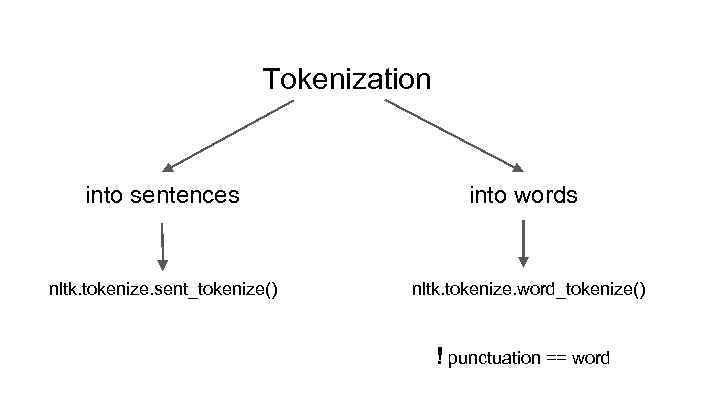
\includegraphics[width=\textwidth]{img1.jpeg}
    \caption{tokenizing}
    \caption*{https://cdn-images-1.medium.com}
    \label{fig:my_label}
\end{figure}

\subsection{Stemming and Lemmatization}
Stemming is a process to eliminate affixes(prefix,suffix,infix,circumfix) from a word in order to obtain a word stem or root word.

going -> go , happily -> happy , am/are/is -> be.

A common term associated with stemming is Lemmatization. There is a slight difference between stemming and Lemmatization

Stemming cuts off the end or beginning of the word,taking into account a list of common prefixes and suffixes

Form : Studies Suffix : es Stem : Studi

Form : Studying Suffix : ing Stem : Study

Lemmatization takes into consideration morphological analysis of the words.

Form : Studies Lemma : Study

Form : Studying Lemma : Study

Lemmatization definitely has an edge over stemming but building a Stemmer is far easy then the latter as deep linguistic knowledge is required to look for the proper form of word.
\chapter{Applications of NLP}
\begin{figure}
    \centering
    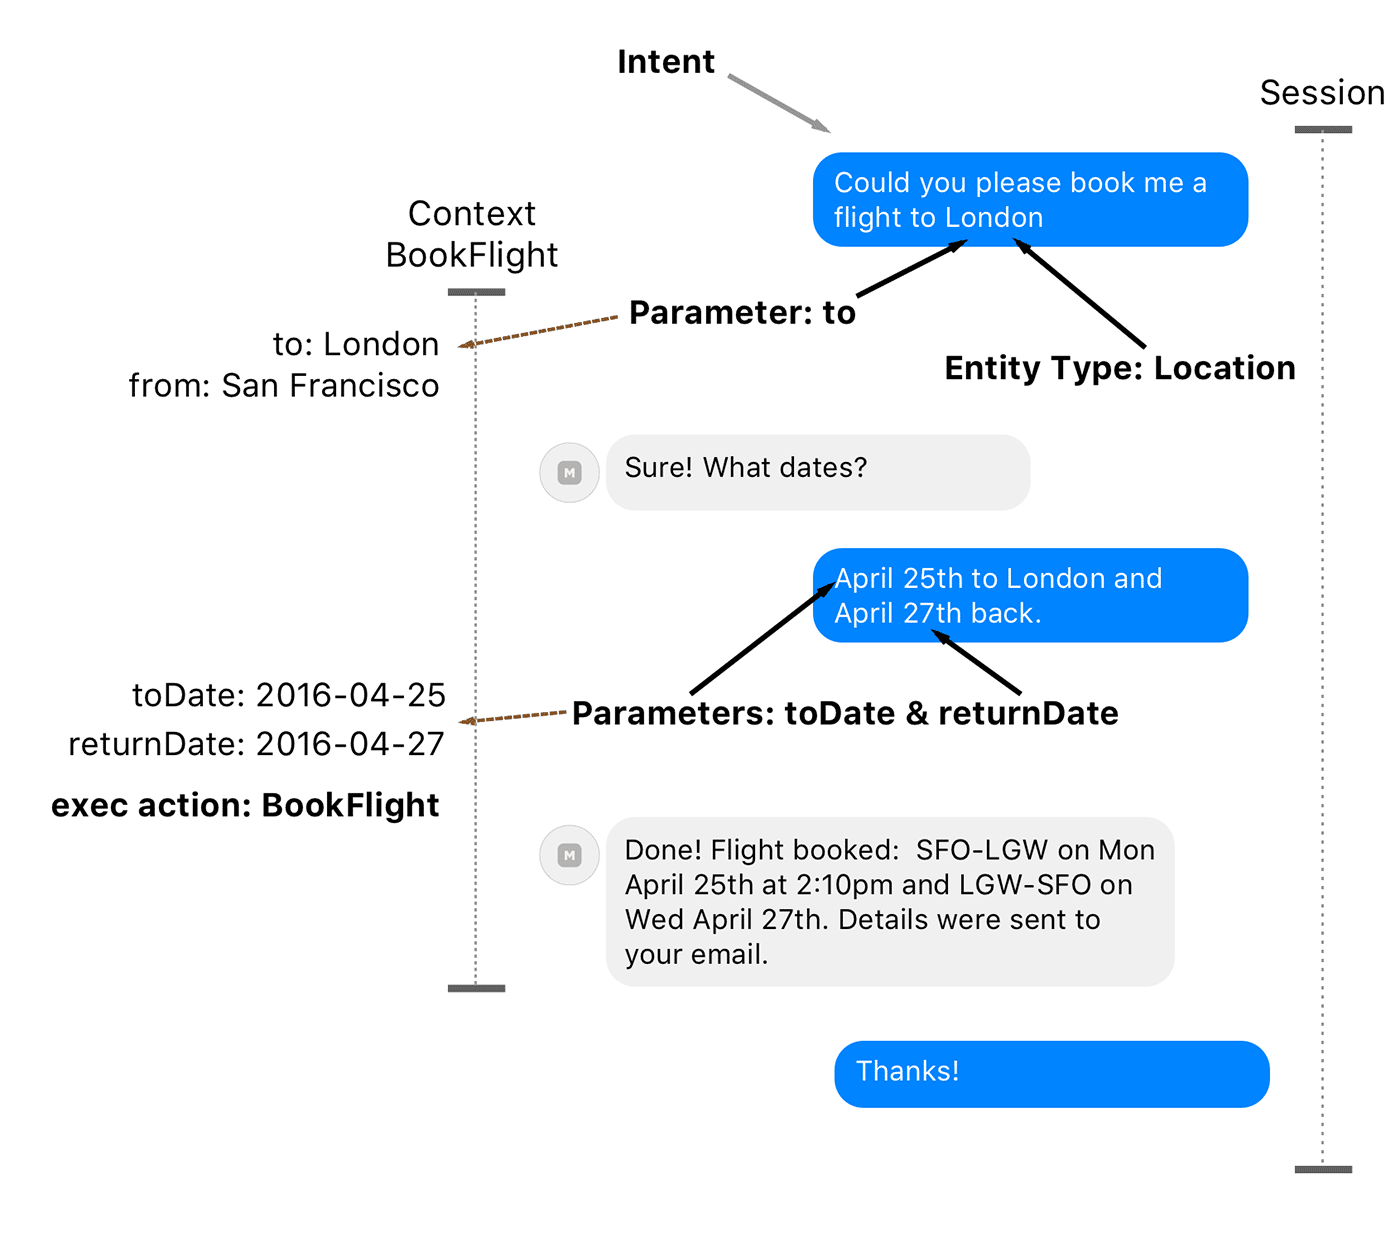
\includegraphics[width=\textwidth]{nlp.png}}
    \caption{Working}
    \caption*{http://www.nlp.com/what-is-nlp/}
    \label{nlp1}
\end{figure}

\begin{itemize}


\item  Text Classification and Categorization\\
Text classification is an essential part in many applications, such as web searching, information filtering, language identification, readability assessment, and sentiment analysis. Neural networks are actively used for these tasks.\\
\item Named Entity Recognition (NER)\\
The main task of named entity recognition (NER) is to classify named entities, such as Guido van Rossum, Microsoft, London, etc., into predefined categories like persons, organizations, locations, time, dates, and so on. Many NER systems were already created, and the best of them use neural networks\\
\item Part-of-Speech Tagging\\
Part-of-speech (POS) tagging has many applications including parsing, text-to-speech conversion, information extraction, and so on. In the work, Part-of-Speech Tagging with Bidirectional Long Short-Term Memory Recurrent Neural Network a recurrent neural network with word embedding for part-of-speech (POS) tagging task is presented \\
\item Semantic Parsing and Question Answering\\
Question Answering systems automatically answer different types of questions asked in natural languages including definition questions, biographical questions, multilingual questions, and so on. Neural networks usage makes it possible to develop high performing question answering systems.\\
\item  Paraphrase Detection\\
Paraphrase detection determines whether two sentences have the same meaning. This task is especially important for question answering systems since there are many ways to ask the same question.Detecting Semantically Equivalent Questions in Online User Forums suggests a method for identifying semantically equivalent questions based on a convolutional neural network.\\
\item  Language Generation and Multi-document Summarization\\
Natural language generation has many applications such as automated writing of reports, generating texts based on analysis of retail sales data, summarizing electronic medical records, producing textual weather forecasts from weather data, and even producing jokes\\
\item  Machine Translation\\
The purpose of Neural-based Machine Translation for Medical Text Domain study is to inspect the effects of different training methods on a Polish-English machine translation system used for medical data. To train neural and statistical network-based translation systems The European Medicines Agency parallel text corpus was used. \\
\item  Character Recognition\\
The article Character Recognition Using Neural Network presents a method for the recognition of handwritten characters.
\end{itemize}
\chapter{Conclusion}
As a computerized approach of analyzing text, NLP is continually striving forward. Researchers are
continually trying to gather knowledge on how human beings understand and use various
languages. This aid in the development of appropriate tools and techniques which make computer
systems understand and manipulate natural languages to perform the various tasks. Technologies,
such as string matching, keyword search, glossary lookup are now on the past as, to more forward
looking technologies such as grammar checkers, conceptual search, event extraction, interlingual on
going and striving forward

\newpage

\begin{verbatim}
[1]E.D. Liddy, Natural Language Processing, 2001 \\
[2]  S.  Vijayarani1,  J.  Ilamathi  and  Nithya,  “Preprocessing  Techniques  for  Text  Mining  -  An Overview”,
\\International  Journal  \\of  Computer  Science  &  Communication  Networks,  Vol.5, issue.1, pp. 7-16 7 ISSN: 2249-578 \\
[3] J.  Wiebe,  E. Breck,  C.  Buckley,  C.  Cardie, P.  Davis,  B.  Fraser,  D. Litman, \\ D.  Pierce,  E. Riloff,  T. Wilson, D. Day, and M. Maybury, \\ 
“Recognizing and Organizing Opinions Expressed in the World Press”. In  \\Proceedings of 2003 AAAI Spring Symposium on New  Directions in Question Answering, 2003. \\
[4] P. Jackson and I. Moulinier,”Natural Language Processing for  Online Applications”: \Cambridge University press, New York.2012, page 7-9.  \\
[5]  R.  Bose.  “Natural  language  processing:  Current  state  and  future  directions”. International Journal of the Computer, the Internet and Management Vol. 12#1 (January –  April, 2004) pp. 1  – 11. 
 
\end{verbatim}

\end{document}

